\chapter{I Was Broke, Found God, and Now I Make \$15M/Year}

This School of Hard Knocks interview, curated by LazyingArt LLC, is not a blackboard lecture, but it still unfolds with a clear mathematical spine. We move from virality and credibility into a chain of sharper claims about attention, money, resilience, economic eras, sales, assets, mentorship, and trust. The useful way to read it is not as a bag of maxims, but as a small system: what we attend to changes what we build; what we build changes what pays us; and what we withdraw too early weakens the entire machine. We will therefore stay close to the order of the conversation and formalize only those relations that the interview itself plainly supports.

\begin{remark}
No validated mathematical screenshots survive for this lecture. Every equation and diagram below is therefore transcript-backed or a cautious editorial reconstruction of what the speaker is doing in words.
\end{remark}

\section{Prologue: Proof, Promise, and the First Filter}

We begin where the interview begins: not with a theory, but with a compressed proof of significance. The opening street-interview montage establishes three claims in rapid sequence. Myron Golden is a consultant and entrepreneur; he has made \$15 million in a single year; and his life includes both earlier poverty and later reversal. Then comes the theological line that the rest of the interview will keep circling back to: he does not merely believe in God, he trusts God.

The host then adds a second layer of credibility. The earlier clip has drawn roughly \(150\) million views across social media. At this point the conversation offers its first slogan,
\begin{equation}
\text{Attention} \rightarrow \text{Revenue}.
\end{equation}
At the beginning this is only a slogan. Later the lecture will give us a more articulated mechanism. But already the host is converting spectacle into instruction. The golf-course meeting is framed not as a casual follow-up, but as a blueprint for becoming a multimillionaire and for learning sales and marketing at eight-figure scale.

The first serious question on the course asks what the wealthiest people do differently. Golden's answer is deliberately spare: they hyper-focus on intention and ignore distraction. The host immediately tries to paraphrase this as a thesis about going deep on one thing and not diversifying, but Golden resists that translation. Diversification, he says, is another conversation. The point here is more primitive. Before we discuss strategy, we need a filter.

\begin{definition}
For any candidate activity \(a\), we may encode Golden's distinction as
\begin{align}
I(a)=1 &\iff a \text{ moves the needle in our favor},\\
D(a)=1 &\iff a \text{ does not move the needle in our favor}.
\end{align}
Here \(I(a)\) records intention and \(D(a)\) records distraction.
\end{definition}

The force of the answer lies in its austerity. The lecture does not begin by teaching us how to multiply channels. It begins by asking whether the thing in front of us belongs at all in the small set of actions that actually advance the objective. Only after that filter is in place does the host ask what money itself is for.

\section{What Money Is For}

The interview preserves the rhythm of spoken conversation here. There is a brief interruption while the group moves across the course; then the host re-enters with, in effect, ``so you were saying.'' Golden answers by widening the frame one step further. Wealthy people, he says, perceive life differently. The first sign of that altered perception is not how much money they have, but what they take the primary purpose of money to be.

Let \(M\) denote money regarded not merely as quantity, but as an object to which one assigns a dominant use. Then the lecture offers a three-part comparison:
\begin{align}
\text{Poor:}\quad & M \mapsto \text{pay bills},\\
\text{Middle class:}\quad & M \mapsto \text{maintain credit and status consumption},\\
\text{Rich:}\quad & M \mapsto \text{turn money into more money}.
\end{align}

This is the hinge of the chapter. The point is not simply that the rich possess more units of \(M\). The point is that they apply a different operator to it. If money is assigned to bill service, it disappears into maintenance. If it is assigned to display, it disappears into social signaling. If it is assigned to reproduction, it is routed into a process that seeks more of itself.

Golden makes the claim concrete at once. When he gets a dollar, he says, he wants to turn it into \(10\), or better into \(100\), or even \(1000\), before spending it. But he immediately adds the mechanism. Money does not multiply by self-adoration. It multiplies when we perceive what is valuable to other people and solve their problem instead of staring only at our own shortage. In the lecture's own order, the wealth chain is
\begin{equation}
\text{perceive value to others}
\rightarrow
\text{solve their problem}
\rightarrow
\text{receive income}
\rightarrow
\text{retain and reinvest}
\rightarrow
\text{asset growth}.
\end{equation}

That is why Golden insists that we cannot be focused on our money problem while solving it. The money problem is solved indirectly. One's attention has to rest on the other person's difficulty; the financial return is the downstream effect of having done that work well.

\section{Survival, Reinvestment, and the Cost of Upgrading Too Early}

The interview now performs a useful test. Do these principles survive biography? Golden corrects himself on the way to the answer, finally saying that he was \(45\) when he made his first million. But what matters more for the lecture is the second half of the story: after making a million dollars a year for a couple of years in a row, he lost all of his money.

The explanation has two layers. One layer is contingency: a series of tragedies. The other is structural and therefore teachable: he upgraded his lifestyle too soon. Here the lecture becomes financial engineering in miniature. If inflow rises and withdrawals rise with it, then the system develops a larger appetite before it has built sufficient reserves. Golden quotes the biblical line that when riches increase, those who consume them increase as well. In commercial terms, that means success recruits expenses very quickly.

Let \(X_t\) denote current inflow, \(C_t\) current consumption or lifestyle withdrawal, \(W_t\) retained wealth, and \(\Pi_t\) the returns produced by retained capital. Golden's benchmark is blunt:
\begin{equation}
C_t \le 0.1X_t.
\end{equation}
He gives this as a rule of thumb: live on \(10\%\) of revenue or income if possible. We should not misread the number \(0.1\) as an optimized theorem. It is a lecture heuristic. But it has real structure, because it separates the cash that sustains the person from the cash that preserves the machine.

At the level of a simple reserve model, if liquid reserves are \(R\) and inflow falls to zero, then runway is approximately
\begin{equation}
T_{\mathrm{runway}} \approx \frac{R}{C_t}.
\end{equation}
This is not stated verbatim in the interview; it is the simplest bookkeeping form of Golden's point.

\paragraph{Worked example.}
Suppose reserves are
\[
R=120{,}000.
\]
If spending is held to
\[
C_t=5{,}000 \quad \text{per month},
\]
then runway is
\[
T_{\mathrm{runway}} \approx \frac{120{,}000}{5{,}000}=24 \text{ months}.
\]
But if the same person upgrades lifestyle so that
\[
C_t=40{,}000 \quad \text{per month},
\]
then the very same reserve buys only
\[
T_{\mathrm{runway}} \approx \frac{120{,}000}{40{,}000}=3 \text{ months}.
\]
This is the lecture's resilience argument in arithmetic form. Lower burn does not merely feel safer; it changes the time scale on which shocks can be survived.

The companion bookkeeping identity is
\begin{equation}
W_{t+1}=W_t+\Pi_t-C_t.
\end{equation}
Again, Golden does not write down this recurrence. But it captures exactly what he is saying: if we are always pulling money out to buy things, the base available for future growth stays small; if withdrawals are restrained, the retained base grows larger, and the next round of gains is computed from a larger stock. His saying, ``stay small enough, long enough, and you'll be big enough soon enough,'' is the verbal summary of this update rule.

\section{Economic Eras, AI, and Objectives Without Deadlines}

From here the lecture widens its lens. Asked what industry he would enter right now, Golden answers immediately: something to do with AI. The explanation is not a technical discussion of models or software. It is a regime argument. It is easier, he says, to create wealth in the economic era one is living in than in a previous one. Wealth migrates, and when it migrates a new era is introduced.

\begin{figure}[h]
\centering
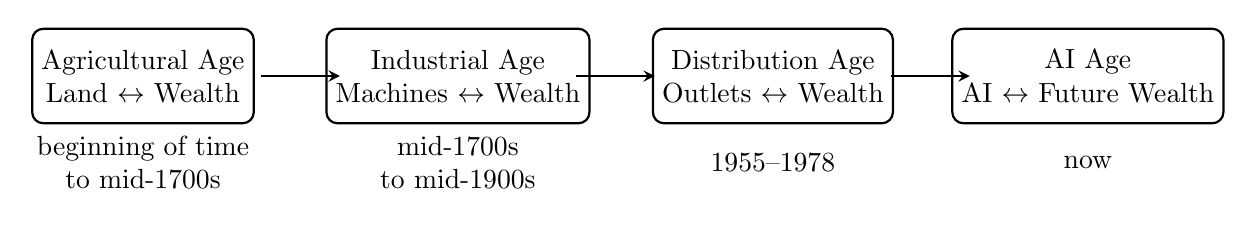
\begin{tikzpicture}[>=stealth,thick]
\node[draw,rounded corners,align=center,minimum width=2.8cm,minimum height=1.2cm] (a) at (0,0) {Agricultural Age\\Land \(\leftrightarrow\) Wealth};
\node[draw,rounded corners,align=center,minimum width=2.8cm,minimum height=1.2cm] (b) at (4.0,0) {Industrial Age\\Machines \(\leftrightarrow\) Wealth};
\node[draw,rounded corners,align=center,minimum width=2.8cm,minimum height=1.2cm] (c) at (8.0,0) {Distribution Age\\Outlets \(\leftrightarrow\) Wealth};
\node[draw,rounded corners,align=center,minimum width=2.8cm,minimum height=1.2cm] (d) at (12.0,0) {AI Age\\AI \(\leftrightarrow\) Future Wealth};
\draw[->] (1.5,0) -- (2.5,0);
\draw[->] (5.5,0) -- (6.5,0);
\draw[->] (9.5,0) -- (10.5,0);
\node[align=center] at (0,-1.1) {beginning of time\\to mid-1700s};
\node[align=center] at (4.0,-1.1) {mid-1700s\\to mid-1900s};
\node[align=center] at (8.0,-1.1) {1955--1978};
\node[align=center] at (12.0,-1.1) {now};
\end{tikzpicture}
\caption{Transcript-derived timeline of wealth regimes. The dates and labels are kept in the rough form in which they are spoken.}
\end{figure}

The chronology is intentionally rough because the interview gives it roughly: agricultural age, where land equaled wealth; industrial age, where machines equaled wealth; distribution age, where outlets equaled wealth; and now the AI age, where those entering AI early help create the wealth of the future. We should not inflate this into a full textbook history. Its role in the lecture is motivational and strategic: it justifies the move from guarding wealth to locating the next zone of wealth formation.

The host then tests the claim with a deadline challenge: if one had to start from zero and make a million dollars in \(90\) days, what would one do? Golden refuses the premise, and the refusal is one of the lecture's clearest conceptual moves.

\begin{definition}
Golden defines a goal by
\begin{equation}
G := O+\tau,
\end{equation}
where \(O\) is an objective and \(\tau\) is a deadline.
\end{definition}

Why refuse the challenge? Because, he says, he does not control deadlines, nor the times and seasons. His analogy is agricultural: one does not force \(7\) million ears of corn by next Wednesday if the crop cycle does not permit it. The lecture therefore replaces deadline pressure with a smaller and more controllable discipline:
\begin{enumerate}
\item choose objectives for inputs,
\item choose objectives for outcomes,
\item omit hard deadlines when the clock is not under one's control.
\end{enumerate}

This should not be mistaken for passivity. The argument is subtler. Uncontrolled deadlines generate false verdicts. One misses the arbitrary clock, feels like a failure, and may quit even though the process was still alive. Golden is trying to remove a self-imposed term that corrupts persistence.

\section{First Sales Move: Desire, Findability, and Ease}

After the macroeconomic detour, the interview narrows again. Asked whether he is a good salesman, Golden answers, without softening it, that he is one of the best in the world. The host immediately asks for the distinguishing habit, and again the answer is simpler than a catalogue of tricks: he sells people things they desire to buy.

That single move strips away the common caricature of selling as pressure. Golden contrasts two postures. In the first, the seller wants somebody to buy simply because something is for sale. In the second, the seller begins with already existing desire in the market and asks how to become visible to it. The crucial line is that there are already millions of people who would love to buy what one would love to sell if only they knew one existed.

Thus the first sales move in the lecture is not force but discoverability. We do not begin by cornering a buyer. We begin by making ourselves findable to buyers who already want the relevant class of solution. Selling becomes easier when the match is prepared in advance by desire.

This section of the conversation remains deliberately elementary. It does not yet move into premium offers, transparent pricing, or large-ticket group sales. Those come later, after the interview has passed through the question of family trajectory and the value of mentorship. But the essential reversal is already on the page: selling works better when we align with desire than when we push against it.

\section{Changing the Family Trajectory}

The host now does something characteristic of the interview: he turns a general principle back toward biography. After discussing sales and market desire, he asks whether Golden came from a rich family and then presses the sharper question: how did he change his family's trajectory?

\subsection{Question \& Answer}

The question is posed against a familiar slogan: the rich get richer, the poor get poorer. Golden's first move is not yet the answer. It is a logical correction:
\begin{equation}
\text{correlation} \neq \text{causation}.
\end{equation}
The rich may get richer and the poor may get poorer, but the first statement does not by itself explain the second. The lecture pauses here because Golden does not want a slogan to masquerade as a mechanism.

His answer then comes in two parts. The first is motive: he hated being poor. The second is method: he learned what rich people did and began doing those things instead of the things poor people did. The most compact line in this part of the lecture is one he attributes to Daniel Priestley:
\begin{equation}
A \rightarrow Y,
\end{equation}
that is, income follows assets.

We should read this as directional and structural, not as a finely estimated law. Golden's claim is that the center of gravity must shift away from wages and bills toward the accumulation of assets. He says this in almost accounting language: he stopped focusing on working hard, on eight hours of work for eight hours of pay, and on paying bills. He started focusing on putting more assets in the asset column.

\begin{figure}[h]
\centering
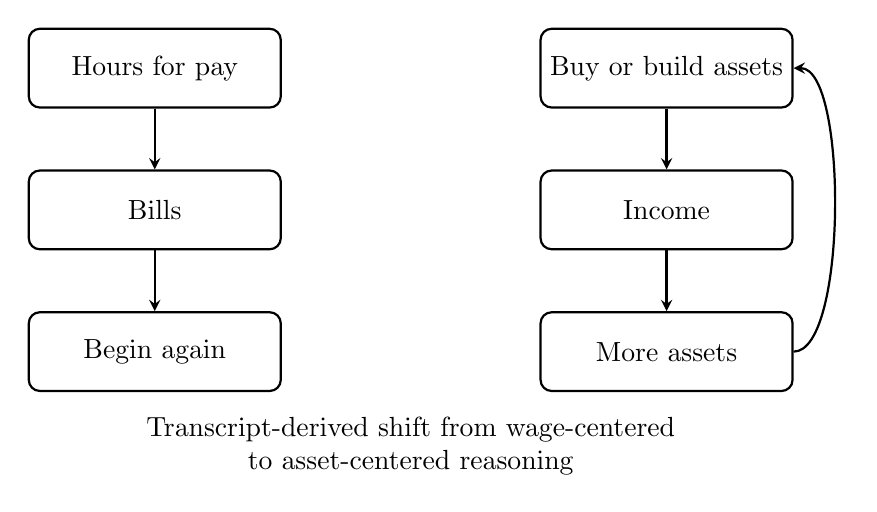
\begin{tikzpicture}[>=stealth,thick]
\node[draw,rounded corners,align=center,minimum width=3.2cm,minimum height=1cm] (l1) at (0,0) {Hours for pay};
\node[draw,rounded corners,align=center,minimum width=3.2cm,minimum height=1cm] (l2) at (0,-1.8) {Bills};
\node[draw,rounded corners,align=center,minimum width=3.2cm,minimum height=1cm] (l3) at (0,-3.6) {Begin again};

\node[draw,rounded corners,align=center,minimum width=3.2cm,minimum height=1cm] (r1) at (6.5,0) {Buy or build assets};
\node[draw,rounded corners,align=center,minimum width=3.2cm,minimum height=1cm] (r2) at (6.5,-1.8) {Income};
\node[draw,rounded corners,align=center,minimum width=3.2cm,minimum height=1cm] (r3) at (6.5,-3.6) {More assets};

\draw[->] (l1) -- (l2);
\draw[->] (l2) -- (l3);

\draw[->] (r1) -- (r2);
\draw[->] (r2) -- (r3);
\draw[->] (r3.east) .. controls (8.8,-3.6) and (8.8,0) .. (r1.east);

\node[align=center] at (3.25,-4.8) {Transcript-derived shift from wage-centered\\to asset-centered reasoning};
\end{tikzpicture}
\caption{The interview's central reorientation: income is not the first object, but the downstream effect of assets.}
\end{figure}

The lecture then makes the asset language concrete. One may buy assets, but one may also build them. Books are the clean example: written once, paid from repeatedly. Later, when the host asks what Golden is investing in now, we hear about real estate options, some crypto, and, most importantly, his own mind. That last remark belongs here because it extends the asset argument one level upward. The mind is not yet the cash flow, but it is part of the mechanism that produces the next asset.

\section{Mentorship, Bigger Thinking, and the Final Return to Sales and Trust}

\paragraph{Mentorship as leverage.}
The interview now turns from assets to learning. Asked how much he has spent on mentorship, Golden answers: about \$1.7 million if one includes books, courses, coaching, and the rest. The point of the number is not drama. It is leverage. Mentorship, in his account, is the ultimate shortcut because someone else has already spent a life figuring out how to do a thing, and one can buy access to the structure of that discovery.

The strongest formulation in this stretch of the lecture is epistemic:
\begin{equation}
\text{the things we do not know we do not know}
\end{equation}
are often the real barrier. Ordinary ignorance is not the only problem; hidden ignorance is the worse one. That is why mentorship has such disproportionate value. It exposes a region of the map we did not even know was missing.

Golden's first mentor, Jerry, showed him how to sell one-to-many from a stage. The anecdote matters because Golden says he did not even believe the method would work until he performed it. Here again the lecture is practical rather than merely inspirational. Often the mind catches up to the method only after the method has already worked.

The Robert G. Allen story then raises the scale of the whole discussion. Golden reports telling Allen that he had gone from being a trash man earning \$6.25 an hour to making \$30,000 a month. Allen's response was that he was doing well and was on the path to making really big money. The shock lies not in the compliment, but in the reframing: \( \$30{,}000 \) a month, which had felt enormous, is suddenly revealed as small relative to a larger field. The lecture's vocabulary here is perception again. One must learn to see the larger structure already there.

\paragraph{After the interruption.}
The interview contains a promotional break in the middle. Once that interruption is omitted, the conversation resumes with a question about credibility and access: how does someone get in the room without already having a great deal of status? Golden's answer is practical and memorable. One pays to be in the room, buys one's way in, and gets paid on the way out. He illustrates this with the story of joining a mastermind as the broke person in the room and discovering, to his surprise, that people far ahead of him financially still saw immense value in his ideas.

That produces a second sales correction. He had been selling to the people who needed what he had, instead of the people who wanted it and would willingly pay for it. Market choice, then, depends on objective. If the objective is to get rich, sell to rich people. If the objective is to solve expensive problems, find the buyers for whom those problems are in fact expensive.

This is also where the lecture re-enters sales at a higher resolution. Golden gives price points not to boast, but to explain market filtration: coaching at \$40,000 an hour, programs in the \$20,000--\$30,000 range, and some offers extending to \$1 million per year. By stating price early, he says, he attracts the right people and repels the wrong ones. The buyer self-selects.

The lecture then provides its most explicit definition of sales.

\begin{definition}
Sales is the uncovering of value so clearly that people are happy to exchange money for what has been revealed.
\end{definition}

This definition explains why his response to resistance is not automatically to lower the price. One may instead ask whether the revealed value is too thin. In the lecture's own logic, pressure is a poor substitute for clarity.

Asked about the most money he has made in a single day, Golden says about \$5.5 million, and he explains it not as a trick but as a premium offer made to a group. At this point the opening slogan about attention is finally refined into a mechanism:
\begin{equation}
\text{Attention}
\rightarrow
\text{Relationship}
\rightarrow
\text{Trust}
\rightarrow
\text{Purchase}
\rightarrow
\text{Investment}.
\end{equation}
This is the meaning of his claim that free value is not really free. People pay first with attention. If they pay with attention long enough, some of them will later pay with assets, which is to say they will invest in themselves through the seller.

\paragraph{The closing frame.}
Only now does the interview make its last return to the line planted in the opening montage: trust in God. Golden's answer is frankly testimonial. He trusts God because, in his account, God has never lied to him; what God says in scripture has proven itself not only true, but truth. We should state this exactly as his claim, not as neutral doctrine.

The financial lesson he draws from scripture is likewise presented as his own interpretation. He quotes the line that the blessing of the Lord makes rich and adds no sorrow with it. He also gives a second principle that reconnects the spiritual material to the whole commercial argument: greatness comes through service. In business, he says, one can be great even without unusual brilliance, provided one is willing to serve enough people, because greatness is the ability to serve the masses.

The final exchange gathers the chapter into a single mood. Life is short, even if one lives to \(100\). One should love the people one loves, fill life with actual experiences, and live with gratitude. The greatest lesson, Golden says, is that everything good in his life is a gift. In the architecture of the interview, this is not an appendix. It is the last interpretive lens through which he wants the earlier claims to be seen: attention, money, sales, assets, and mentorship all sit inside a theology of service, gift, and trust.

\section{Summary}

The interview begins as proof, becomes a blueprint, and ends as a theology of wealth. Along the way it gives us a compact but coherent system. First, filter attention: intention moves the needle and distraction does not. Second, redefine the purpose of money: not merely bill service, but the production of more money. Third, protect the system with low burn, because early consumption shortens runway and weakens compounding. Fourth, locate the present regime of wealth creation rather than fighting the previous one. Fifth, understand sales as alignment with desire and, later, as the clear revelation of value. Sixth, treat poverty escape not as a slogan about class dynamics, but as a shift from wages toward assets. Seventh, use mentorship to expose the ignorance we cannot yet see.

None of this is presented as pure technique. The lecture keeps turning technique into structure, and structure into posture. Wealth, in Golden's account, is built by solving problems, retaining enough to survive, placing oneself in the right era and the right rooms, choosing the right market, and learning to perceive abundance where one had previously seen only scarcity. The final note of the chapter is therefore fitting: the machine is commercial, but the horizon in which he understands it is moral and theological.